\documentclass[11pt,oneside]{article}

\pdfminorversion=7
\usepackage{QuizStyle}
\usepackage{tikz}

\hypersetup{
    pdftitle={20261119 Quiz for MATH102 Calculus II},
    pdfauthor={Jungwoo Kim},
    pdfsubject={Quiz for MATH102 Calculus II},
    pdfcreator={LaTeX}
}

\begin{document}

\quiztitle{20261119 Quiz}

\begin{problem}{6.24}
Compute
\[
    \iint_D f(x,y)\,\dd A,
\]
where $D$ is the region bounded by the lines $y=1$, $x=y$, and
$x=4-y$, and $f(x,y)=e^{x+y}$.
\end{problem}
\begin{solution}
The lines $x=y$ and $x=4-y$ meet at $(2,2)$, while $y=1$ meets
them at $(1,1)$ and $(3,1)$. Hence
\[
    D=\{(x,y)\in\R^2\mid 1\le y\le2,\ y\le x\le4-y\}.
\]
Integrating first with respect to $x$, we obtain
\[
\begin{aligned}
    \iint_D e^{x+y}\,\dd A
    &=\int_1^2\int_y^{4-y}e^{x+y}\,\dd x\,\dd y\\
    &=\int_1^2\left(e^4-e^{2y}\right)\,\dd y\\
    &=\left[e^4y-\frac12e^{2y}\right]_1^2
     =\boxed{\frac{e^4+e^2}{2}}.
\end{aligned}
\]
\end{solution}

\begin{problem}{6.25}
Evaluate
\[
    \iint_D y\,\dd A,
\]
where $D$ is the upper half-disk $x^2+y^2\le1$, $y\ge0$.
\end{problem}
\begin{solution}
For each $-1\le x\le1$, the variable $y$ ranges from $0$ to
$\sqrt{1-x^2}$. Therefore
\[
\begin{aligned}
    \iint_D y\,\dd A
    &=\int_{-1}^{1}\int_0^{\sqrt{1-x^2}}y\,\dd y\,\dd x\\
    &=\frac12\int_{-1}^{1}(1-x^2)\,\dd x\\
    &=\frac12\left[x-\frac{x^3}{3}\right]_{-1}^{1}
     =\boxed{\frac23}.
\end{aligned}
\]
\end{solution}

\begin{problem}{6.26}
Evaluate the integrals.
\begin{problemsubparts}
    \item $\displaystyle\iint_D(x^2-y^2)\,\dd A$,
          where $D=[-1,1]\times[0,2]$.
    \item $\displaystyle\iint_D x^2y^2(x+y)\,\dd x\,\dd y$,
          where $D=[0,1]\times[0,1]$.
\end{problemsubparts}
\end{problem}
\begin{solution}
\begin{problemsubparts}
    \item By iterated integration,
    \[
    \begin{aligned}
        \iint_D(x^2-y^2)\,\dd A
        &=\int_{-1}^1\int_0^2(x^2-y^2)\,\dd y\,\dd x\\
        &=\int_{-1}^1\left(2x^2-\frac83\right)\,\dd x
         =\boxed{-4}.
    \end{aligned}
    \]
    \item Expanding the integrand and separating the integrals gives
    \[
    \begin{aligned}
        \iint_D x^2y^2(x+y)\,\dd x\,\dd y
        &=\left(\int_0^1x^3\,\dd x\right)
          \left(\int_0^1y^2\,\dd y\right)\\
        &\quad+\left(\int_0^1x^2\,\dd x\right)
          \left(\int_0^1y^3\,\dd y\right)\\
        &=\frac14\cdot\frac13+\frac13\cdot\frac14
         =\boxed{\frac16}.
    \end{aligned}
    \]
\end{problemsubparts}
\end{solution}

\begin{problem}{6.29}
Evaluate
\[
    \iint_R\sin y\,\dd A,
\]
where $R$ is the region $0\le x\le1$, $0\le y\le\sqrt{x}$.
\end{problem}
\begin{solution}
The inequality $y\le\sqrt{x}$ is equivalent to $x\ge y^2$,
and $0\le y\le1$. Thus reversing the order of integration gives
\[
\begin{aligned}
    \iint_R\sin y\,\dd A
    &=\int_0^1\int_{y^2}^1\sin y\,\dd x\,\dd y\\
    &=\int_0^1(1-y^2)\sin y\,\dd y.
\end{aligned}
\]
Integration by parts yields
\[
    \int y^2\sin y\,\dd y
    =-y^2\cos y+2y\sin y+2\cos y.
\]
Consequently,
\[
\begin{aligned}
    \iint_R\sin y\,\dd A
    &=\left[-\cos y+y^2\cos y
           -2y\sin y-2\cos y\right]_0^1\\
    &=\boxed{3-2\sin1-2\cos1}.
\end{aligned}
\]
\end{solution}

\begin{problem}{6.30}
Evaluate
\[
    \iint_R xe^y\,\dd A,
\]
where $R$ is the region bounded by $y=x+2$ and $y=x^2$.
\end{problem}
\begin{solution}
The curves intersect where $x^2=x+2$, that is, at
$x=-1$ and $x=2$. Since $x^2\le x+2$ between these points,
\[
\begin{aligned}
    \iint_R xe^y\,\dd A
    &=\int_{-1}^2\int_{x^2}^{x+2}xe^y\,\dd y\,\dd x\\
    &=\int_{-1}^2x\left(e^{x+2}-e^{x^2}\right)\,\dd x.
\end{aligned}
\]
Using $\int xe^{x+2}\,\dd x=(x-1)e^{x+2}$ and
$\int xe^{x^2}\,\dd x=\frac12e^{x^2}$, we obtain
\[
\begin{aligned}
    \iint_R xe^y\,\dd A
    &=\left[(x-1)e^{x+2}-\frac12e^{x^2}\right]_{-1}^2\\
    &=\boxed{\frac{e^4+5e}{2}}.
\end{aligned}
\]
\end{solution}

\begin{problem}{6.32}
Consider the mapping
\[
    \begin{pmatrix}x\\y\end{pmatrix}
    =\begin{pmatrix}1&1\\0&1\end{pmatrix}
     \begin{pmatrix}u\\v\end{pmatrix}.
\]
\begin{problemsubparts}
    \item Show that the Jacobian is $1$.
    \item Sketch the triangle with vertices $(1,0)$, $(1,1)$, and $(0,1)$,
          and its image under the mapping. Show that its image has the same area.
\end{problemsubparts}
\end{problem}
\begin{solution}
The mapping is $\mathbf F(u,v)=(u+v,v)$.
\begin{problemsubparts}
    \item Its derivative matrix is
    \[
        D\mathbf F(u,v)=\begin{pmatrix}1&1\\0&1\end{pmatrix},
        \qquad
        \boxed{\det D\mathbf F(u,v)=1}.
    \]
    \item The vertices are mapped as follows:
    \[
        (1,0)\mapsto(1,0),\qquad
        (1,1)\mapsto(2,1),\qquad
        (0,1)\mapsto(1,1).
    \]
    The original triangle has horizontal and vertical legs of length $1$.
    Its image also has a horizontal leg of length $1$ and a vertical leg
    of length $1$, as shown below.

    \begin{center}
    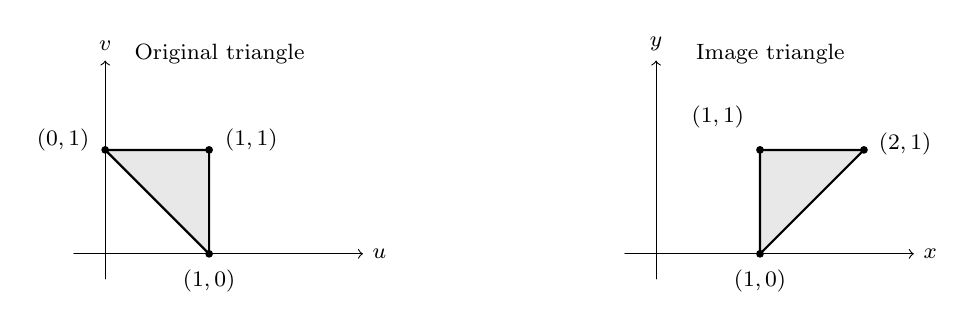
\begin{tikzpicture}[x=1.32cm,y=1.32cm,
                        every node/.style={font=\footnotesize},
                        line cap=round,line join=round]
      \begin{scope}
        \draw[->,thin] (-0.30,0)--(2.48,0) node[right] {$u$};
        \draw[->,thin] (0,-0.24)--(0,1.86) node[above] {$v$};
        \fill[black!9] (1,0)--(1,1)--(0,1)--cycle;
        \draw[thick] (1,0)--(1,1)--(0,1)--cycle;
        \fill (1,0) circle (1.4pt);
        \fill (1,1) circle (1.4pt);
        \fill (0,1) circle (1.4pt);
        \node[below] at (1,-0.06) {$(1,0)$};
        \node[right] at (1.06,1.10) {$(1,1)$};
        \node[left] at (-0.06,1.10) {$(0,1)$};
        \node at (1.10,1.92) {Original triangle};
      \end{scope}
      \begin{scope}[shift={(5.30,0)}]
        \draw[->,thin] (-0.30,0)--(2.48,0) node[right] {$x$};
        \draw[->,thin] (0,-0.24)--(0,1.86) node[above] {$y$};
        \fill[black!9] (1,0)--(2,1)--(1,1)--cycle;
        \draw[thick] (1,0)--(2,1)--(1,1)--cycle;
        \fill (1,0) circle (1.4pt);
        \fill (2,1) circle (1.4pt);
        \fill (1,1) circle (1.4pt);
        \node[below] at (1,-0.06) {$(1,0)$};
        \node[right] at (2.05,1.06) {$(2,1)$};
        \node[above left] at (0.94,1.12) {$(1,1)$};
        \node at (1.10,1.92) {Image triangle};
      \end{scope}
    \end{tikzpicture}
    \end{center}
    Both triangles therefore have area
    \[
        \boxed{\operatorname{Area}=\frac12}.
    \]
    This agrees with the Jacobian $|\det D\mathbf F|=1$.
\end{problemsubparts}
\end{solution}

\begin{problem}{6.34}
For a mapping of the form $(x,y)=(f(u),g(v))$, verify that the
Jacobian is given by
\[
    \det\begin{pmatrix}x_u&x_v\\y_u&y_v\end{pmatrix}
    =f'(u)g'(v).
\]
\end{problem}
\begin{solution}
Since $x=f(u)$ depends only on $u$ and $y=g(v)$ only on $v$,
\[
    x_u=f'(u),\quad x_v=0,\quad y_u=0,\quad y_v=g'(v).
\]
Hence the derivative matrix is diagonal, and its determinant is
\[
    \boxed{\det\begin{pmatrix}x_u&x_v\\y_u&y_v\end{pmatrix}
      =\det\begin{pmatrix}f'(u)&0\\0&g'(v)\end{pmatrix}
      =f'(u)g'(v)}.
\]
\end{solution}

\begin{problem}{6.37}
Use the change of variables $(x,y)=(r\cos\theta,r\sin\theta)$
to polar coordinates to evaluate
\[
    \iint_D e^{-\|\mathbf X\|}\,\dd A,
\]
where $D$ is the set of points $(x,y)$ with
$a^2\le x^2+y^2\le b^2$, and $a,b$ are positive constants.
\end{problem}
\begin{solution}
When $a\le b$, the region is the annulus $a\le r\le b$.
Since $\|\mathbf X\|=r$ and the absolute value of the polar
Jacobian is $r$, the change of variables formula gives
\[
\begin{aligned}
    \iint_D e^{-\|\mathbf X\|}\,\dd A
    &=\int_0^{2\pi}\int_a^b e^{-r}r\,\dd r\,\dd\theta\\
    &=2\pi\left[-(r+1)e^{-r}\right]_a^b\\
    &=\boxed{2\pi\left((a+1)e^{-a}-(b+1)e^{-b}\right)}.
\end{aligned}
\]
If $a>b$, then $D$ is empty and the integral is $0$.
\end{solution}

\begin{problem}{6.38}
Use symmetries or the change of variables
$(x,y)=(r\cos\theta,r\sin\theta)$ to evaluate the integrals,
where $D$ is the annulus
\[
    1\le\sqrt{x^2+y^2}\le8.
\]
\begin{problemsubparts}
    \item $\displaystyle\iint_D(x^2+y^2)^p\,\dd A$,
          where $p$ is any number.
    \item $\displaystyle\iint_D(3+y-x^2)\,\dd A$.
    \item $\displaystyle\iint_D\ln(x^2+y^2)\,\dd A$.
\end{problemsubparts}
\end{problem}
\begin{solution}
The polar description of the annulus is $1\le r\le8$,
$0\le\theta\le2\pi$, and $\dd A=r\,\dd r\,\dd\theta$.
\begin{problemsubparts}
    \item For every real $p$,
    \[
        \iint_D(x^2+y^2)^p\,\dd A
        =\int_0^{2\pi}\int_1^8r^{2p+1}\,\dd r\,\dd\theta
        =2\pi\int_1^8r^{2p+1}\,\dd r.
    \]
    If $p\ne-1$, this gives
    \[
        \boxed{\frac{\pi}{p+1}\left(8^{2p+2}-1\right)}.
    \]
    If $p=-1$, the radial integrand is $1/r$, and the value is
    \[
        \boxed{2\pi\ln8}.
    \]
    \item The integral of $y$ over $D$ vanishes by symmetry.
    Moreover,
    \[
    \begin{aligned}
        \iint_D3\,\dd A
        &=3\pi(8^2-1^2)=189\pi,\\
        \iint_Dx^2\,\dd A
        &=\int_0^{2\pi}\cos^2\theta\,\dd\theta
          \int_1^8r^3\,\dd r\\
        &=\pi\cdot\frac{8^4-1}{4}
         =\frac{4095\pi}{4}.
    \end{aligned}
    \]
    Therefore
    \[
        \boxed{\iint_D(3+y-x^2)\,\dd A
        =189\pi-\frac{4095\pi}{4}
        =-\frac{3339\pi}{4}}.
    \]
    \item Since $x^2+y^2=r^2$, the substitution $t=r^2$
    gives
    \[
    \begin{aligned}
        \iint_D\ln(x^2+y^2)\,\dd A
        &=2\pi\int_1^8r\ln(r^2)\,\dd r\\
        &=\pi\int_1^{64}\ln t\,\dd t\\
        &=\pi\left[t\ln t-t\right]_1^{64}\\
        &=\boxed{\pi\left(64\ln64-63\right)}.
    \end{aligned}
    \]
\end{problemsubparts}
\end{solution}

\end{document}
